\documentclass{article}
\usepackage[spanish]{babel}
\usepackage[utf8]{inputenc}
\usepackage[T1]{fontenc}
\usepackage{vmargin}
\usepackage{setspace}
\usepackage{enumerate}
\usepackage{graphicx}
\graphicspath{ {images/} }
\usepackage{float} 

\begin{document}
\begin{center}
\includegraphics[scale=0.5]{unison1.jpg}
\\
\vspace{0.5cm}
UNIVERSIDAD DE SONORA \\
\vspace{0.5cm}
DIVISIÓN DE CIENCIAS EXACTAS Y NATURALES \\
\vspace{0.5cm}
DEPARTAMENTO DE FÍSICA\\
\vspace{0.5cm}
LICENCIATURA EN FÍSICA\\
\vspace{0.5cm}
FÍSICA COMPUTACIONAL I

\vspace{2 cm}
\hrule
\vspace{1 cm}

{\huge \bfseries {Reporte de actividad 2}}
\\

\vspace{1 cm}
\hrule
\vspace{2 cm}
Ricardo Ruiz Hernández\\ 
\vspace{1 cm}
Profesor del curso\\
Dr. Carlos Lizárraga Celaya\\
\vspace{2 cm}
07 de febrero del 2018
\end{center}

\pagebreak
\begin{doublespace}

\hrule
\section{Introducción}
El manejo de datos, así como la graficación de los mismos, son los temas principales que se abordan en el desarrollo de esta práctica. Para cumplir con la actividad recurrimos a uno de los lenguajes de programación más utilizados en la actualidad: Python. 

¿Qué es Python? 
Python es un lenguaje de programación poderoso y fácil de aprender. Cuenta con estructuras de datos eficientes y de alto nivel y un enfoque simple pero efectivo a la programación orientada a objetos. La elegante sintaxis de Python y su tipado dinámico, junto con su naturaleza interpretada, hacen de éste un lenguaje ideal para scripting y desarrollo rápido de aplicaciones en diversas áreas y sobre la mayoría de las plataformas.

El entorno utilizado fue el de Jupyter Notebook, el cual es una aplicación web que permite crear y compartir documentos que contienen código fuente, ecuaciones, visualizaciones y texto explicativo. Entre sus usos está la limpieza y transformación de datos, la simulación numérica, el modelado estadístico, el aprendizaje automático y mucho más.
\vspace{0.5 cm}
\hrule
\vspace{0.6 cm}
\section{Actividad}
El primer paso fue correr Jupyter Notebook desde la terminal, lo que abrió una pestaña nueva llamada Home en el navegador, desde ahí iniciamos una sesión en Python.
Trabajamos con un conjunto de datos brindados por el sitio del Sistema Meoteorológico Nacional de alguna localidad; en mi caso, escogí la colonia Ecoguardas del Distrito Federal.
Se nos brindó acceso a un ejemplo en un repositorio, colocado con el profesor; en tal ejemplo estaba descrito un código que debíamos imitar, remplanzando los datos con los nuestros, que para ese momento, ya debían de estar en el repositorio.

\subsection{Código}
\begin{itemize}
\item La primer celda contenía el código que se encargaría de cargar las bibliotecas con las que se trabajarían,   (panda, numpy y matplotlib), el código fue el siguiente:
\begin{center}
\textit{import pandas as pd \\ import numpy as np \\ import matplotlib.pyplot as plt}
\end{center}

\item Se cargaron los datos de Ecoguardas con el siguiente comando: 
\textit{df0 = pd.read\_csv('LaMalinche.txt', skiprows=4, sep='\char`\\ s+')}

\item Una vez plamados los primeros 5 renglones de nuestros datos (utilizando el código \textit{df0.head()}), se procedió a darle una estructura de data frame (utilizamos el comando \textit{df = pd.DataFrame(df0)}) 
\item Acto seguido se presentaron los tipos de datos que Pandas ha reconocido al leer, para ello, introducimos el siguiente comando: \textit{df.dtypes}

\item Convertimos a variable de tiempo la combinación de las columnas DD/MM/AAAA y HH:MM, para también dentro de la misma celda eliminar las primeras dos columnas que ya no necesitábamos.
\item Los siguientes pasos nos ilustraron como obtener promedios y análisis exploratorios:
\begin{center}
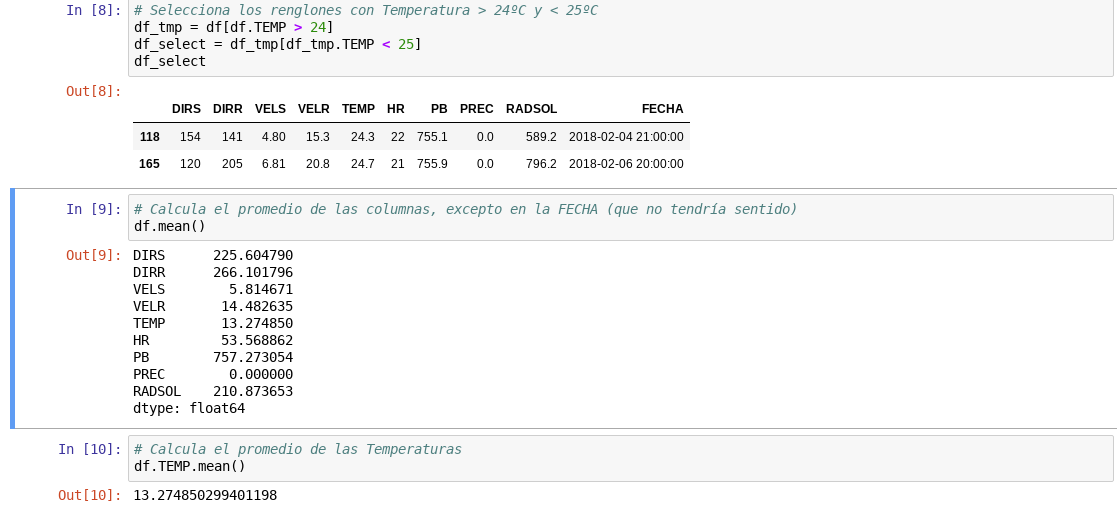
\includegraphics[scale=0.5]{promedios.png}
\end{center}

\item Finalmente, se exponen códigos para hacer gráficas:
\\
-Gráfica de la rapidez de los vientos:
\\
\includegraphics[scale=0.5]{Gr_fica1.png}

-Gráfica de temperatura y humedad relativa:
\\
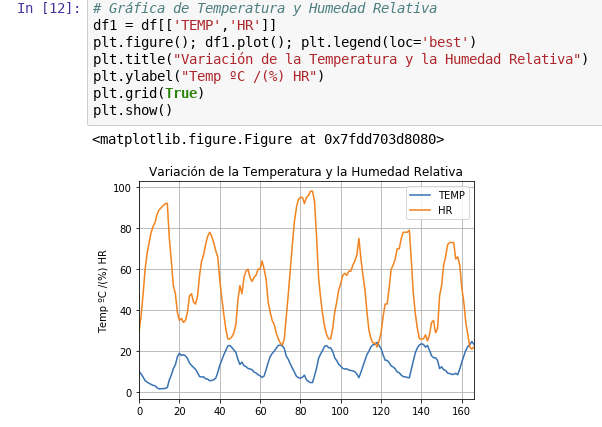
\includegraphics[scale=0.5]{grafica2.png}
\\
-Gráfica de la variación de la temperatura:
\\
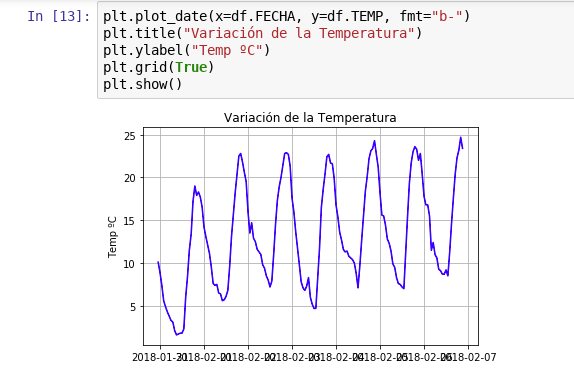
\includegraphics[scale=0.5]{grafica3.png}

\subsection{Indicaciones adicionales}
Tomando como referencia todo lo anterior, se nos indicó graficar: la rapidez de los vientos y la rapidez de las ráfagas como funciones del tiempo. 

\item Muestro las tres gráficas a continuación, en el orden que fueron mencionadas:
\\
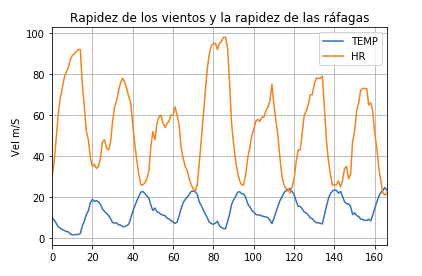
\includegraphics[scale=0.5]{grafica4.png}
\\
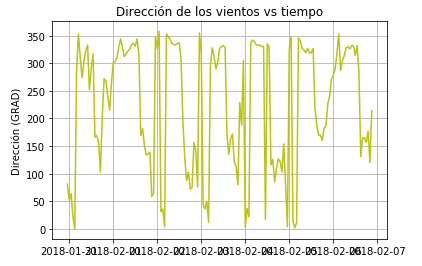
\includegraphics[scale=0.5]{grafica5.png}
\\
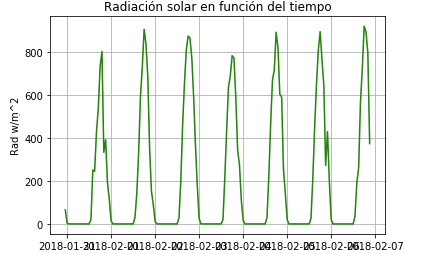
\includegraphics[scale=0.5]{grafica6.png}
\\
\item En base a lo anterior se plantea la pregunta: ¿Cuál es el lapso de temperatura diaria?, y para responderla, hice uso de un comando para calcular la diferencia entre la temperatura máxima y la mínima: \textit{df1=df[['TEMP']]} y
\textit{df1.max()-df1.min()}. Siendo el resultado de 23.1 grados.

\item Seguidamente se nos indica que se realice el análisis exploratorio de datos, que resuma el sitio estudiado (Usar la función describe() sobre tu data frame. El resultado de aplicar este comando fue el siguiente:
\\
\begin{center}
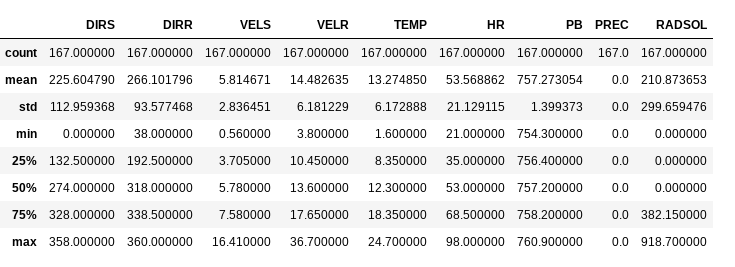
\includegraphics[scale=0.5]{ultimatabla.png}
\end{center}

\subsection{Apéndice}
\begin{enumerate}
\item ¿Cuál es tu primera impresión de Jupyter Notebook?
\\
Me pareció muy amena, puesto que comparando este entorno con FORTRAN (de nuestro anterior curso de programación), hace todo mucho más fluido y sencillo, sobre todo por el hecho de no tener que compilar el programa en cada momento.

\item ¿Se te dificultó leer código en Python?
\\
La dificultad de algo nuevo, conforme me fui adentrando, esa dificultad disminuyó.
\item ¿En base a tu experiencia de programación en Fortran, que te parece el entorno de trabajar en Python?
\\
Como mencioné recién, más cómodo. Jupyter Notebook se encargó de facilitar la programación.
\item A diferencia de Fortran, ahora se producen las gráficas utilizando la biblioteca Matplotlib. ¿Cómo fue tu experiencia?
\\
Me llevo un gran sabor de boca, puesto que, siendo nuestra primera experiencia con este lenguaje, graficamos; en contraste con Fortran, donde la realización de gráficas fue prácticamente nula.
\item En general, ¿qué te pereció el entorno de trabajo en Python? 
\\
Me pareció un buen entorno, del cual quiero aprender mucho más.
\item ¿Qué opinas de la actividad? ¿Estuvo compleja? ¿Mucho material nuevo? ¿Que le faltó o que le sobró? ¿Qué modificarías para mejorar? 
\\
La actividad cumple con su cometido, introducirnos a este nuevo entorno de Phyton y Jupyter Notebook; sin embargo, me pareció algo compleja de realizar, por el hecho de desconocer en su mayoría este lenguaje. No me parece que sea mucho material, simplemente uno debe de analizar a fondo e investigar sobre los comandos, de esta manera, no debe de haber un gran problema para realizar dicha sesión.

\item ¿Comentarios adicionales que desees compartir? 
\\
Phyton parece ser lo que se dice, un lenguaje ameno y elegante, del cual seguiré aprendiendo con entusiasmo a lo largo de este curso.

\end{enumerate}

\section{Conclusión}

El manejo de este nuevo lenguaje de programación (para nosotros como estudiantes), debe y representa un gran avance en nuestro caminar por el mundo de la ciencia, puesto que es bien sabido, que la programación es fundamental en el presente y futuro. En lo que concierne a Jupyter Notebook, es poseedor de muchas bondades, estas lo hacen un entorno de programación atractivo, en el que, da gusto trabajar. Esta actividad nos permitió tener un panorama más amplio de lo que Phyton y Jupyter Notebook son.

\section{Bibliografía}
\textit{$https://live.osgeo.org/es/quickstart/jupyter_quickstart.html$}
\\
\textit{$https://desarrolloweb.com/articulos/1325.php$}


\end{itemize}
\end{doublespace}
\end{document}


